\documentclass[12pt]{article}

\usepackage{sbc-template}
\usepackage{graphicx,url}
\usepackage[utf8]{inputenc}
\usepackage[brazil]{babel}
\usepackage{booktabs}

\sloppy

\title{Avaliação Exploratória de um Modelo Compacto de \emph{Tool-Calling}
para Interfaces de Comando em Português no Contexto de IoT Apícola}

\author{}
\address{}

\begin{document}

\maketitle


\begin{resumo}
Sistemas de IoT para colmeias tipicamente exigem comandos de sintaxe fixa,
uma barreira para operadores sem formação técnica. Avaliamos de forma
exploratória o Needle 2, modelo de \textit{tool-calling} de 45M de
parâmetros executável offline em microcontrolador, como interface de
comando em português para IoT apícola. Validamos a execução do modelo em
hardware real (ESP32-S3 N16R8) e avaliamos sistematicamente 36 casos em
português no motor de referência do projeto, cobrindo comandos diretos,
variações coloquiais, parâmetros implícitos, ambiguidade e frases fora de
escopo. O modelo atingiu 36,1\% de acurácia exata, com forte assimetria
entre comandos diretos (75,0\%) e casos com nuance ou recusa (16,7\% a
25,0\%), e sua confiança reportada não se mostrou suficiente como rede de
segurança contra erros de ferramenta.
\end{resumo}



\begin{abstract}
IoT beehive-monitoring systems typically require fixed-syntax commands, a
barrier for operators without technical training. We present an
exploratory evaluation of Needle 2, a 45M-parameter \textit{tool-calling}
model that runs offline on a microcontroller, as a Portuguese command
interface for apiculture IoT. We validate the model execution on real
hardware (ESP32-S3 N16R8) and systematically evaluate 36 Portuguese cases
on the project's reference engine, covering direct commands, colloquial
phrasing, implicit parameters, ambiguity, and out-of-scope phrases. The
model achieved 36.1\% exact-match accuracy, with strong asymmetry between
direct commands (75.0\%) and cases requiring nuance or refusal (16.7\% to
25.0\%), and its reported confidence was not sufficient as a safety net
against tool-selection errors.
\end{abstract}


\section{Introdução}

A aplicação de IoT ao monitoramento de colmeias vem sendo estudada como forma de reduzir a necessidade de inspeções manuais frequentes \cite{henry2019precision,meikle2015application}, especialmente em contextos de agricultura familiar no semiárido, onde a distância entre propriedades e a instabilidade da conectividade podem dificultar a supervisão remota. Sistemas desse tipo geralmente disponibilizam dados e configurações por meio de painéis web ou comandos seriais de sintaxe fixa. Embora essas interfaces sejam adequadas para desenvolvedores, podem dificultar a operação em campo por usuários sem formação técnica, que precisam memorizar comandos específicos ou navegar por telas de configuração em dispositivos móveis, muitas vezes sob conectividade limitada ou inexistente.

Modelos de linguagem poderiam, em princípio, fornecer uma interface baseada em linguagem natural para esse tipo de operação. Entretanto, modelos convencionais apresentam requisitos computacionais incompatíveis com os microcontroladores utilizados nesses sistemas embarcados e, em geral, dependem de serviços em nuvem para inferência. Essa dependência é particularmente problemática em cenários de operação com conectividade instável. Nesse contexto, modelos compactos de \textit{tool-calling} capazes de executar localmente em microcontroladores oferecem uma alternativa para a interpretação de comandos em linguagem natural sem conexão externa. O Needle 2~\cite{ndubuaku2026controlled,cactusneedle2repo}, com 45M de parâmetros e uma pegada de memória de aproximadamente 28MB, é um exemplo recente dessa categoria. Seus benchmarks públicos, entretanto, concentram-se majoritariamente no inglês, sem avaliação específica em português ou em um domínio agrícola.

O Needle 2 \cite{ndubuaku2026controlled} utiliza uma arquitetura denominada pelos autores de \textit{Simple Attention Network}, com Hadamard MLP, atenção por grupos de consultas (GQA) e uma memória de chave-valor baseada em hashing (\textit{engram}). Os pesos são quantizados desde o pré-treinamento por meio da técnica Cactus Quants (CQ2-bit), resultando em um binário de aproximadamente 14~MB que requer cerca de 28~MB de RAM para uma sessão completa, sem necessidade de GPU ou NPU \cite{cactusneedle2repo}. O projeto também disponibiliza um mecanismo de \textit{fine-tuning} local baseado em LoRA, permitindo a adaptação dos
pesos para tarefas ou domínios específicos sem recompilar o motor de
inferência.

Com aproximadamente 45 milhões de parâmetros, o Needle 2 possui porte
inferior a outros modelos compactos de \textit{function-calling} citados
pelos autores, como FunctionGemma (270M) e LFM2.5 (230M). Trabalhos como
TinyAgent \cite{erdogan2024tinyagent} também investigam a especialização
de modelos compactos para \textit{function-calling} por meio de
\textit{fine-tuning}. Esses resultados motivam investigar até que ponto
um modelo de porte reduzido pode executar chamadas estruturadas em
cenários específicos, como comandos em português para aplicações IoT.

A interface avaliada neste trabalho recebe comandos em texto, e não
diretamente em áudio. Embora o hardware utilizado disponha de microfone
integrado, seu uso não faz parte do escopo desta avaliação e é considerado
como possibilidade de trabalho futuro. Soluções como a ESP-SR
\cite{espressif2026espsr} permitem reconhecimento local de palavras-chave
em dispositivos ESP32, mas operam com vocabulários previamente definidos.
Neste trabalho, o interesse está na interpretação de diferentes
formulações textuais em linguagem natural para sua conversão em chamadas
estruturadas de ferramentas.

No contexto da apicultura de precisão, sistemas baseados em sensores
permitem acompanhar variáveis como peso, temperatura e umidade das
colmeias \cite{henry2019precision,meikle2015application,danieli2024precision}.
Neste trabalho, o interesse está na camada de interação com esses sistemas, investigando a conversão de comandos em português em chamadas estruturadas de ferramentas, e não no processamento ou na análise dos sinais coletados. Revisões recentes sobre apicultura de precisão destacam que a adoção dessas tecnologias envolve, além do sensoriamento, aspectos relacionados à usabilidade e à interação com o produtor \cite{danieli2024precision}. Nesse contexto, este trabalho investiga de forma exploratória o uso do Needle 2 como interface local de comando em português para um cenário de IoT aplicado à apicultura. O estudo concentra-se em um cenário ainda pouco explorado: a utilização de um modelo compacto de \textit{tool-calling}, executável em microcontrolador, para interpretar comandos em português associados a operações de monitoramento apícola.

As principais contribuições deste trabalho são: (1) a definição de um
\textit{schema} com três ferramentas representativas de operações no
domínio apícola; (2) a construção de um conjunto de teste com 36 frases
em português brasileiro, abrangendo comandos diretos, variações
coloquiais, parâmetros ausentes ou vagos, ambiguidades e frases fora de
escopo; e (3) uma avaliação exploratória do Needle 2 nesse cenário,
combinando a validação de sua execução em hardware real (ESP32-S3 N16R8)
com a coleta sistemática dos 36 casos no motor host de referência. O
estudo não inclui validação em campo com apicultores nem integração com
sensores físicos de uma colmeia. Essas limitações são discutidas na
Seção~\ref{sec:discussao}.

O restante deste artigo está organizado da seguinte forma:
a Seção~\ref{sec:metodologia} descreve a proposta, o ambiente experimental, o \textit{schema} de ferramentas, o conjunto de teste e o protocolo de avaliação; a Seção~\ref{sec:resultados} apresenta os resultados quantitativos e qualitativos; a Seção~\ref{sec:discussao} discute as implicações dos resultados e as limitações do trabalho; e a
Seção~\ref{sec:conclusao} apresenta as conclusões.

\section{Metodologia}
\label{sec:metodologia}

\subsection{Proposta}
\label{sec:proposta}

A proposta consiste em utilizar um modelo compacto de
\textit{tool-calling} como camada de interpretação entre comandos em
linguagem natural e operações de um sistema de monitoramento apícola.
Foram definidas três ferramentas representativas de consultas e ações
nesse domínio, mantendo o \textit{schema} reduzido diante do orçamento de
contexto do modelo. A Figura~\ref{fig:fluxo} apresenta o fluxo proposto:
o comando em texto é submetido ao modelo, que produz uma chamada de
ferramenta compatível com o \textit{schema} ou uma chamada vazia quando
nenhuma das operações disponíveis é aplicável.


\begin{figure}[h]
	\centering
	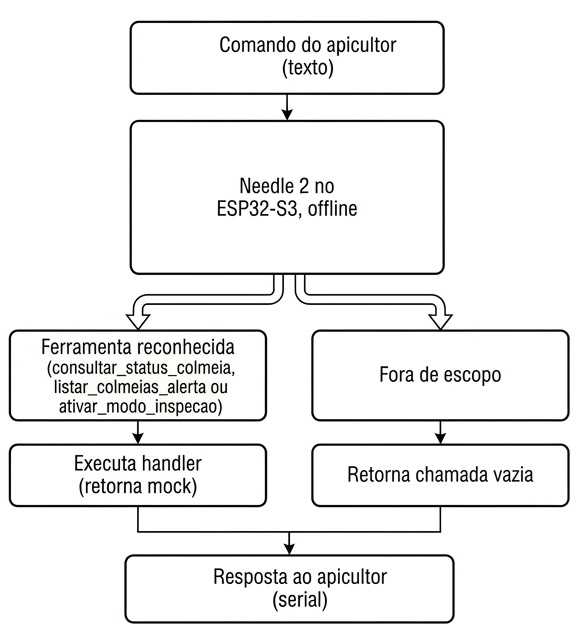
\includegraphics[width=0.6\textwidth]{fluxo_proposta.jpg}
	\caption{Fluxo de funcionamento do comando por linguagem natural.}
	\label{fig:fluxo}
\end{figure}

As operações definidas representam funcionalidades compatíveis com
sistemas de monitoramento apícola baseados em sensores de peso,
temperatura e umidade, entre outras variáveis
\cite{henry2019precision,meikle2015application,danieli2024precision,cota2023bhivesense}. A proposta não modifica a camada de sensoriamento, mas acrescenta uma camada de interação responsável por converter comandos em linguagem natural em chamadas estruturadas de ferramentas.

Nesta etapa, os \textit{handlers} utilizam dados simulados, uma vez que a
integração com sensores físicos não faz parte do escopo experimental.
Dessa forma, a avaliação concentra-se na capacidade do modelo de
interpretar os comandos e produzir as chamadas de ferramentas esperadas.

\subsection{Hardware e ambiente}

O hardware-alvo é uma placa ESP32-S3-WROOM-1 N16R8 (16~MB de flash e
8~MB de PSRAM em modo octal), configuração compatível com os requisitos
do motor de referência utilizado \cite{cactusneedle2repo}. O firmware foi
compilado com ESP-IDF v5.5.5 e sua execução foi validada nesse hardware
antes da coleta sistemática do conjunto de teste. O processo de
inicialização, incluindo o carregamento do modelo \texttt{needle2.cact} e
o \textit{priming} inicial do prefixo do \textit{schema}, levou 52,3,s.
A taxa de decodificação observada foi de 553\,ms/token, correspondente a
aproximadamente 1,81 tokens/s. Esses resultados demonstram a execução do
modelo na configuração de hardware utilizada e fornecem a caracterização
temporal do ambiente embarcado considerado neste estudo.


A coleta sistemática dos 36 casos foi realizada no motor host do projeto
(binário \texttt{nd\_dump}), compilado a partir do mesmo código-fonte C
utilizado pelo firmware embarcado. O motor foi executado em Linux (WSL2
sobre Windows), em uma CPU convencional. Essa escolha decorreu de
instabilidades observadas na comunicação via USB-CDC durante os testes
preliminares no Windows e permitiu realizar a coleta sem depender da
interface serial. A Figura~\ref{fig:fluxo} apresenta o procedimento
experimental e distingue a validação no hardware-alvo da coleta realizada
no motor host. As diferenças entre os ambientes são consideradas na
análise da latência, conforme discutido na
Seção~\ref{sec:discussao}.


\subsection{Schema de ferramentas}

O schema foi limitado a três ferramentas, dado o orçamento de contexto de
256 tokens do modelo \cite{ndubuaku2026controlled}:
\texttt{consultar\_status\_colmeia(colmeia\_id)},
\texttt{listar\_colmeias\_alerta()} e
\texttt{ativar\_modo\_inspecao(colmeia\_id, duracao\_min)}. Os nomes dos parâmetros e suas descrições foram definidos com vocabulário
relacionado ao domínio apícola, incluindo termos como peso, temperatura,
alerta e inspeção. O \textit{schema} foi fornecido ao motor em formato
JSON compactado, sem espaços em branco, conforme recomendado pela
documentação do projeto de referência, com o objetivo de reduzir o uso de
tokens de formatação desnecessários.

\subsection{Conjunto de teste}

O conjunto de teste é composto por 36 frases em português brasileiro,
construídas manualmente e associadas previamente às respostas esperadas.
Os casos foram distribuídos em cinco categorias: comandos diretos (N=8);
variações de fala coloquial e numerais por extenso (N=8); parâmetros
ausentes ou vagos (N=6), destinados a verificar se o modelo evita
preencher argumentos não fundamentados no comando; frases ambíguas
(N=6), incluindo referências a múltiplas colmeias, referências espaciais
sem identificador numérico e solicitações mais específicas do que as
operações disponíveis; e frases fora de escopo (N=8), para as quais se
espera uma chamada de ferramenta vazia.

As categorias foram definidas para representar diferentes níveis de
complexidade de interpretação e incluir casos limite relevantes para a
avaliação. Os casos com parâmetros ausentes, ambiguidades e entradas fora
de escopo permitem avaliar, além da seleção da ferramenta, a capacidade
do modelo de evitar argumentos não fundamentados e chamadas indevidas.

\subsection{Protocolo experimental e métricas}

Cada uma das 36 frases foi executada uma única vez no motor host. Dessa
forma, os resultados caracterizam o comportamento observado em uma
execução do conjunto de teste, sem estimar a variabilidade entre
repetições. Essa escolha é tratada como uma limitação do estudo
exploratório e considerada na interpretação dos resultados, conforme
discutido na Seção~\ref{sec:discussao}. O modo de raciocínio explícito do
modelo (\texttt{!think}) foi desabilitado (\texttt{nothink}) em todas as
execuções, de forma a avaliar diretamente a saída produzida pelo modelo.
Cada execução invocou o motor como um novo processo, sem reutilização de
uma sessão previamente inicializada. Consequentemente, a latência
reportada inclui o custo de \textit{priming} do prefixo do \textit{schema}
em cada chamada.

Cada resposta foi comparada manualmente com o resultado esperado (nome da
ferramenta e argumentos), definido previamente no próprio conjunto de
teste, e classificada em uma das seguintes categorias: acerto exato
(ferramenta e todos os argumentos obrigatórios corretos, além da ausência
correta de argumentos opcionais não fundamentados); acerto parcial
(ferramenta correta, mas com algum argumento incorreto, indevidamente
ausente ou não fundamentado); erro (ferramenta incorreta); rejeição
correta (chamada vazia esperada e obtida); rejeição incorreta (chamada
vazia esperada, mas o modelo produziu uma chamada); e saída múltipla não
prevista, utilizada quando o modelo produziu mais de uma chamada válida
para um caso cujo gabarito não previa esse formato de resposta.


\section{Resultados}
\label{sec:resultados}

\begin{table}[h]
\centering
\caption{Métricas agregadas por categoria de comando (motor host, N=36).}
\label{tab:metricas}
\begin{tabular}{lccc}
\toprule
Categoria & N & Acurácia exata & Latência média (s) \\
\midrule
Diretos              & 8 & 75,0\% (6/8)  & 2,87 \\
Variações de fala     & 8 & 37,5\% (3/8)  & 2,87 \\
Parâmetro implícito   & 6 & 16,7\% (1/6)  & 2,86 \\
Ambíguos              & 6 & 16,7\% (1/6)  & 2,91 \\
Fora de escopo (rejeição correta) & 8 & 25,0\% (2/8) & 2,75 \\
\midrule
\textbf{Geral}        & \textbf{36} & \textbf{36,1\% (13/36)} & \textbf{2,85} \\
\bottomrule
\end{tabular}
\end{table}

A latência permaneceu estável entre as categorias (2,75,s a 2,91,s), sem
relação aparente com a dificuldade dos comandos. No protocolo adotado,
cada execução iniciou um novo processo e, portanto, incluiu novamente o
custo de \textit{priming} do prefixo do \textit{schema}. Essa
característica reduz a influência relativa do comprimento ou da
complexidade linguística da frase sobre o tempo total medido.


\subsection{Padrões de erro qualitativos}

Três padrões sistemáticos foram identificados na inspeção manual dos 36 casos, conforme descrito a seguir.

\textbf{Numerais por extenso não são convertidos.} Nos casos que continham números escritos por extenso (por exemplo, ``colmeia dois'' e ``colmeia número oito''), o modelo não converteu o numeral e preencheu \texttt{colmeia\_id} com o valor 1 (casos 9, 10 e 15). A repetição desse comportamento sugere uma limitação na interpretação de numerais por extenso em português, possivelmente relacionada à tokenização ou aos dados utilizados no treinamento do modelo.

\textbf{Preenchimento de parâmetro ausente.} Nos casos destinados a verificar se o modelo omite um campo não fundamentado no texto (categoria \texttt{parametro\_implicito}, além dos casos análogos 6, 13 e 27), o modelo preencheu \texttt{duracao\_min} com o valor 13 em diferentes situações (casos 6, 10, 13, 17, 21 e 27). A recorrência do mesmo valor em contextos sem relação textual aparente sugere a existência de um valor de preenchimento padrão. Esse comportamento é relevante para o domínio, pois, em um dispositivo real, utilizar uma duração de inspeção não especificada em vez de solicitar esclarecimento poderia resultar em uma ação física não pretendida sobre a colmeia.

\textbf{Rejeição de comandos fora de escopo.} Das 8 frases fora do domínio, o modelo produziu uma chamada vazia em apenas 2 casos (25\%). Nos outros 6, gerou chamadas de ferramentas válidas, principalmente \texttt{consultar\_status\_colmeia} com \texttt{colmeia\_id:1}. Esse comportamento difere do mecanismo de rejeição descrito pelos autores do modelo para entradas em inglês \cite{ndubuaku2026controlled} e pode indicar uma menor capacidade de rejeição para entradas em português. No entanto, essa hipótese requer avaliação adicional com um conjunto de dados maior e controles específicos de idioma.

Também foi observado um comportamento não previsto pelo protocolo de
avaliação no caso 23 (`Colmeia 3 e colmeia 4, como estão?''). O modelo
retornou duas chamadas de \texttt{consultar\_status\_colmeia}, uma com
\texttt{colmeia\_id:3} e outra com \texttt{colmeia\_id:4}. Embora ambas
as chamadas sejam individualmente compatíveis com a solicitação, o
\textit{schema} e o gabarito adotados não previam uma resposta composta
por múltiplas chamadas. Por esse motivo, o caso não foi contabilizado
como acerto exato nem classificado como erro de ferramenta ou de
parâmetro, sendo registrado separadamente como `saída múltipla não
prevista''. A confiança reportada nesse caso foi de 98,47\%.


\subsection{Confiança reportada como sinal de erro}
\label{sec:confianca}

O motor de referência reporta, para cada resposta gerada, uma pontuação de
confiança, pensada como mecanismo de segurança para decidir quando uma
ação deveria ser executada automaticamente ou submetida a confirmação
humana \cite{ndubuaku2026controlled}. A Tabela~\ref{tab:confianca} agrega
essa pontuação pelos quatro desfechos possíveis observados no conjunto de
teste.

\begin{table}[h]
\centering
\caption{Confiança média reportada pelo modelo, por tipo de desfecho (N=36).}
\label{tab:confianca}
\begin{tabular}{lcc}
\toprule
Desfecho & N & Confiança média \\
\midrule
Acerto exato                          & 13 & 88,9\% \\
Erro de parâmetro (ferramenta certa)  & 7  & 17,4\% \\
Erro de ferramenta                    & 15 & 55,7\% \\
Saída múltipla não prevista (caso 23) & 1  & 98,47\% \\
\midrule
\textbf{Total}                        & \textbf{36} & --- \\
\bottomrule
\end{tabular}
\end{table}

As quatro categorias somam o total de 36 casos do conjunto de teste. O
caso 23, já discutido na Seção~\ref{sec:resultados} por produzir duas
chamadas de ferramenta simultâneas em vez de uma, foi isolado como
categoria própria em vez de forçado em alguma das outras três: ele não é
um acerto exato (o schema não previa múltiplas chamadas), não é um erro
de parâmetro nem de ferramenta (ambas as ferramentas identificadas e seus
argumentos individuais estavam corretos). Sua confiança (98,47\%) foi
alta, consistente com o padrão observado nos casos 18, 22, 24 e 25: alta
confiança não se restringe a respostas corretas no formato esperado pelo
schema.

O padrão observado foi assimétrico. Nos casos classificados como erro de
parâmetro, nos quais a ferramenta selecionada estava correta, a confiança
média foi de 17,4\%. Nos erros de ferramenta, entretanto, a confiança
média de 55,7\% apresentou elevada variação: 4 dos 15 casos desse grupo
(casos 18, 22, 24 e 25) apresentaram confiança superior a 0,98, próxima
à observada em respostas corretas. Além disso, a saída múltipla não
prevista do caso 23 apresentou confiança de 98,47\%, reforçando que
valores elevados de confiança também podem ocorrer em respostas que não
satisfazem o protocolo de execução definido.

Considerando, de forma exploratória, um limiar hipotético de confiança de
0,90, abaixo do qual o sistema solicitaria confirmação humana antes de
executar uma ação, 4 dos 15 erros de ferramenta (26,7\%) ainda seriam
aceitos automaticamente. Por outro lado, 4 dos 13 acertos exatos (30,8\%)
seriam submetidos desnecessariamente à confirmação. O caso 23 também
ultrapassaria esse limiar, embora sua saída múltipla não estivesse prevista pelo protocolo. Esses resultados indicam que, no cenário avaliado, a pontuação de confiança não é suficiente, quando utilizada isoladamente, como mecanismo de segurança para decidir pela execução automática de chamadas de ferramenta.



\section{Discussão}
\label{sec:discussao}
\subsection{Generalização para o português e para o domínio apícola}

Os três padrões de erro descritos na Seção~\ref{sec:resultados} --- não
conversão de numerais por extenso, preenchimento de valores não
fundamentados no comando e rejeição fraca de entradas fora de escopo ---
evidenciam uma queda de desempenho nas situações que exigem maior
interpretação linguística. Enquanto os comandos diretos alcançaram
75,0\% de acurácia exata, as categorias envolvendo parâmetros implícitos,
ambiguidade e rejeição apresentaram resultados entre 16,7\% e 25,0\%.

Os benchmarks públicos associados ao modelo concentram-se
majoritariamente em inglês \cite{ndubuaku2026controlled}. Assim, os
resultados obtidos são compatíveis com a hipótese de que diferenças de
idioma e de domínio contribuam para as falhas observadas. Entretanto, o
desenho experimental deste estudo não permite isolar os efeitos do
idioma, do domínio e da própria capacidade do modelo. Uma avaliação
comparativa utilizando conjuntos equivalentes em português e inglês,
assim como testes antes e após adaptação ao domínio, seria necessária
para investigar separadamente esses fatores.

O resultado geral de 36,1\% também pode ser contextualizado por estudos
sobre generalização de \textit{tool-calling} fora do domínio de
treinamento. Um estudo recente sobre falhas de seleção de ferramenta
reporta acurácia de 26\% em cenário fora de domínio, contra 57\% a 74\%
no mesmo sistema em cenário dentro do domínio
\cite{lookingnotpicking2026}. No Berkeley Function-Calling Leaderboard
\cite{bfclv4}, modelos de pequeno porte (0,6B a 3B de parâmetros, ainda
substancialmente maiores que os 45M do Needle 2) apresentam desempenho
consideravelmente inferior ao de modelos de fronteira. Essas comparações
devem ser interpretadas apenas como contexto, uma vez que os protocolos,
modelos e conjuntos de teste não são diretamente equivalentes aos
utilizados neste trabalho. Os resultados obtidos, portanto, caracterizam
as limitações do checkpoint avaliado neste cenário específico, sem
permitir atribuí-las exclusivamente ao idioma, ao domínio ou à
arquitetura do modelo.


\subsection{Interpretação da latência}

A latência média de 2,85,s por requisição (Tabela~\ref{tab:metricas}) foi
medida no motor host, com cada execução iniciando um novo processo e,
consequentemente, realizando novamente o \textit{priming} do prefixo do
\textit{schema}. Em uma sessão persistente de uso do firmware embarcado,
esse custo é realizado uma única vez no início da sessão. No hardware-alvo
real (ESP32-S3 N16R8), o \textit{priming} medido levou 52,3,s e a taxa de
decodificação observada foi de 1,81 tokens/s. Considerando, apenas como
estimativa, uma resposta de aproximadamente 59 tokens, o tempo de geração
seria da ordem de 30 a 35,s, substancialmente superior ao observado no
motor host.

Assim, os valores de latência apresentados na Tabela~\ref{tab:metricas}
caracterizam exclusivamente o ambiente host e não devem ser interpretados
como estimativa direta do tempo de resposta no ESP32-S3. A medição da
latência fim a fim em sessões persistentes no hardware real permanece
necessária para avaliar a usabilidade temporal da abordagem em condições
de operação embarcada.


\subsection{Limitações}

Este trabalho apresenta limitações que devem ser consideradas na
interpretação dos resultados. Primeiro, os \textit{handlers} das
ferramentas utilizam dados simulados, sem integração com uma estação real
de monitoramento de colmeias. Segundo, o conjunto de teste contém 36
frases construídas manualmente e avaliadas a partir de um gabarito
previamente definido, sem validação com apicultores ou revisão por
múltiplos anotadores. Terceiro, cada frase foi executada uma única vez, o
que impede estimar a variabilidade do comportamento do modelo entre
repetições. Quarto, a coleta sistemática foi realizada no motor host;
portanto, os valores de latência reportados não representam diretamente o
tempo de resposta no hardware-alvo. Por fim, foi utilizado o checkpoint
público do modelo sem \textit{fine-tuning} ou adaptação específica ao
português e ao domínio apícola. Essas limitações restringem a
generalização dos resultados e caracterizam o estudo como uma avaliação
exploratória do comportamento do modelo no cenário considerado.



\section{Conclusão}
\label{sec:conclusao}

Este trabalho avaliou de forma exploratória o Needle 2, um modelo compacto
de \textit{tool-calling} de 45M de parâmetros, como interface de comando em português para um cenário de IoT apícola. A execução do modelo foi validada em hardware real (ESP32-S3 N16R8), enquanto a avaliação sistemática foi realizada com 36 casos de teste no motor de referência do projeto. O modelo atingiu acurácia exata de 36,1\% no conjunto completo, com desempenho consideravelmente superior em comandos diretos (75,0\%) em comparação com variações coloquiais, parâmetros implícitos e ambiguidades (16,7\% a 37,5\%). A rejeição de comandos fora de escopo apresentou taxa de apenas 25,0\%, evidenciando uma limitação relevante para aplicações nas quais uma interpretação incorreta pode resultar na execução de uma ação não pretendida.

Os resultados também mostraram que a confiança reportada pelo modelo não é, isoladamente, suficiente como mecanismo de segurança, uma vez que foram
observados erros de seleção de ferramenta associados a níveis elevados de
confiança. Em conjunto, os resultados caracterizam as limitações do
checkpoint avaliado para comandos em português no domínio apícola, embora
o desenho experimental não permita atribuí-las exclusivamente ao idioma,
ao domínio ou à capacidade do modelo.

Como trabalhos futuros, pretende-se investigar a adaptação do modelo com um corpus de comandos apícolas em português, integrar os \textit{handlers} a dados reais de monitoramento, realizar avaliações com apicultores e medir a latência fim a fim em sessões persistentes no hardware-alvo. Também se pretende explorar o uso do microfone presente no hardware para uma futura interface de voz. A execução local do modelo em um ESP32-S3 demonstra a possibilidade de empregar modelos compactos de \textit{tool-calling} em microcontroladores, mas os resultados obtidos indicam que o checkpoint avaliado ainda não apresenta confiabilidade suficiente para operação autônoma no cenário considerado.



\bibliographystyle{sbc}
\bibliography{referencias}

\end{document}
